\chapter{Gaussian Process Regression} \label{ch:GaussianProcessRegression}

% **************************** Define Graphics Path **************************
\ifpdf
    \graphicspath{{Chapter3/Figs/Raster/}{Chapter3/Figs/PDF/}{Chapter3/Figs/}}
\else
    \graphicspath{{Chapter3/Figs/Vector/}{Chapter3/Figs/}}
\fi

\section{Brief History of Gaussian Process}
The Gaussian processes is one of the most simple and widely used families of stochastic processes for modelling dependent data observed over time, or space, or time and space together. As a general setting, Gaussian processes of many types have been studied and incorporated in research for decades.
%L$\acute{e}$vy process
The Wiener process (e.g. \cite{Papoulis:1991}) (one of the best known L\'{e}vy processes) is a particular type of Gaussian process. The story of using Gaussian process is still a long one. \cite{Kolmogorov:1941} and \cite{Wiener:1949} used Gaussian process for time series prediction date backs to the 1940's. But probably the history of Gaussian process is even older. The Brownian motion is a Gaussian process. This is because the distribution of a random vector is a linear combination of vector which have a normal distribution. Thorvald N. Thiele was the first to propose the mathematical theory of Brownian motion. He also introduce the likelihood function during the period 1860-1870 when he was serving as a assistant to professor H. L. d'Arrest at the Copenhagen Observatory, Denmark. 

Since the 1970's Gaussian process have been widely adopted in the field of meteorology and geostatistics. Around that time Gaussian process regression was named as kriging and used by \cite{Matheron:1973} for prediction in geostatistics. \cite{O'Hagan:1978} used Gaussian process in the field of statistics for multivariate input regression problem. For general purpose function approximators \cite{Bishop:1995} used neural networks, \cite{Neal:1996} showed the link between Gaussian process and neural networks and in the machine learning context \cite{Williams_and_Rasmussen:1996} first described Gaussian process regression. 

Over the last two decades Gaussian process in machine learning has turned to a major interest and much work has been done. \cite{Rasmussen_and_Williams:2006} perhaps the most widely used and cited article on Gaussian process for machine learning and most of the discussed in this chapter can be found there in detailed form.

%----------------------------------------------------------------------------------------

\section{The Regression Problem}
Machine learning problems can be roughly categorized into three basic classes. 
\begin{enumerate}
 \item Supervised learning: inferring a function from labelled training data
 \item Unsupervised learning: to find hidden structure of unlabelled data 
 \item Reinforcement learning: take action by maximizing the cumulative reward. 
\end{enumerate}
Supervised learning may be further sub-categorized in two fundamental tasks: regression and classification. Regression problem deals with estimating the relationship among some dependent variables with some independent variables, whereas classification identifies the desired discrete output levels. \cite{MacKay:2003}, \cite{Bishop:2006} describes the concepts in detail.

Regression is the task of making some prediction of a continuous output variable at a desired input, based on a training input output data set. The input data can be any type of object or real valued features located in $\mathbb{R}^D$ which have some predictability for an unobserved location. 

By definition of regression, it is obvious that there will be some inference based on a function mapping the outputs from a set of given inputs, because by inferring a function we can predict the response for a desired input. In the case of Bayesian inference, a prior distribution over function is required. Then the model go through some training process and update the prior, based on the training data set $\mathcal{D}$ constructed with $N$ input vectors, such as $\{\textbf{X},\textbf{y}\}$, 
where $\textbf{X}\equiv{\{{\textbf{x}_n}\}_{n=1}^N}$, $ \textbf{x}_n\in\mathbb{R}^D $ 
are the training inputs and 
$\textbf{y}\equiv{\{{y_n}\}_{n=1}^N}$, $ \textbf{y}_i\in\mathbb{R}$
are the training outputs. Now a key question arises, how can we consider a distribution over an infinite dimensional object as a function?

Although using plain and simple statistics regression problem can be solved, but to model a more complex and specific learning task with improved reliability and robustness Gaussian process is a better selection. Gaussian process models can be used for regression model having an object featuring infinite dimensionality. Even Gaussian process have been advanced beyond the regression model and also using for classification(\cite{Williams:1998, Nickisch:2008}), unsupervised learningcite (\cite{Ek:2008}), reinforcement learning (\cite{Deisenroth:2012}) and many more.

We assume the outputs considered at the training level may contain some noise and observed from the underlying mapping function $f(\textbf{x})$. The objective of the regression problem is to construct $f(\textbf{x})$ from the data $\mathcal{D}$. This task is ill-defined and dealing with noisy data leads to an exercise in reasoning under uncertainty. Hence, a single estimate of $f(\textbf{x})$ clearly could be misleading, rather a probability distribution over likely functions could be much more appealing. A regression model based on Gaussian process is a fully probabilistic Bayesian model, and definitely will serve for our purpose. In contrast with other regression models, here we will get the opportunity to choose the best estimate of $f(\textbf{x})$. If we consider a probability distribution on functions $p(f)$ as the Bayesian prior for regression, then from data Bayesian inference can be used to make predictions:
\begin{equation} \label{eq:2.1}
p(f|\mathcal{D})= \frac{p(\mathcal{D}|f)p(f)}{p(\mathcal{D})} 
\end{equation}

% TODO The dynamic activity of transcription factors can be viewed as a regression task.

\section{Gaussian Process definition}
A Gaussian process is a collection of random variables, any finite number of which have a joint Gaussian distribution (\cite{Rasmussen_and_Williams:2006}). It is a continuous stochastic process and defines probability distributions for functions. It can be also viewed as a random variables indexed by a continuous variable: $ f(\textbf{x})$ chosen from a random function variables $ \textbf{f} = \{ f_1, f_2, f_3,..., f_N\}$, with corresponding indexed inputs $ \textbf{X} = \{ \textbf{x}_1, \textbf{x}_2, \textbf{x}_3,..., \textbf{x}_N\}$. In Gaussian processes, variables from these random functions are normally distributed and as a whole can be represent as a multivariate Gaussian distribution:
\begin{equation} \label{eq:2.2}
p(\textbf{f}|\textbf{X})= \mathcal{N}(\boldsymbol\mu,\textbf{K}),
\end{equation}
where $\boldsymbol\mu$ is the mean and $\textbf{K}$ is covariance of Gaussian distribution $\mathcal{N}(\boldsymbol\mu,\textbf{K})$ The Gaussian distribution is over vectors but the Gaussian process is over functions.

We need to define the mean function and covariance function for a Gaussian process prior. If $f(\textbf{x})$ is a real process, a Gaussian process is completely defined by its mean function and covariance function given in equation \ref{eq:2.3} and equation \ref{eq:2.4} respectively. Usually the mean function $m(\textbf{x})$  and the covariance function $k(\textbf{x},\textbf{x\textprime})$ are defined as-
\begin{equation} \label{eq:2.3}
m(\textbf{x})= \mathbb{E}[f(\textbf{x})],
\end{equation}
\begin{equation} \label{eq:2.4}
k(\textbf{x},\textbf{x\textprime})= 
\mathbb{E}[(f(\textbf{x})-m(\textbf{x}))(f(\textbf{x}\textprime)-m(\textbf{x}\textprime))],
\end{equation}
where $\mathbb{E}$ represents the expected value. We denote the Gaussian process as-
\begin{equation} \label{eq:GP}
f\left(\textbf{x} \right)\sim \mathcal{GP} \left(m \left(\textbf{x}\right), k \left(\textbf{x},\textbf{x\textprime}\right) \right).
\end{equation}

The covariance matrix $\textbf{K}$ is constructed from the covariance function $k(\textbf{x},\textbf{x\textprime})$ and $\textbf{K}_{ij}=k\left(\textbf{x}_i,\textbf{x}_j\right)$, that is 
\begin{equation} \label{eq:GP_cov_mat}
\textbf{K} = 
 \begin{pmatrix}
  k\left(\textbf{x}_1,\textbf{x}_1\right) & k\left(\textbf{x}_1,\textbf{x}_2\right) & \cdots & k\left(\textbf{x}_1,\textbf{x}_n\right) \\
  k\left(\textbf{x}_2,\textbf{x}_1\right) & k\left(\textbf{x}_2,\textbf{x}_2\right) & \cdots & k\left(\textbf{x}_2,\textbf{x}_n\right) \\
  \vdots  & \vdots  & \ddots & \vdots  \\
  k\left(\textbf{x}_n,\textbf{x}_1\right) & k\left(\textbf{x}_n,\textbf{x}_2\right) & \cdots & k\left(\textbf{x}_n,\textbf{x}_n\right)
 \end{pmatrix}
\end{equation}
In general, a Gaussian Process is multivariate Gaussian distribution to an infinite number of dimension. A sample from a Gaussian process is a random function. While a $n-$dimensional Gaussian distribution is fully specified by mean $\boldsymbol\mu$, a $n \times 1$ vector of expectations and covariance matrix $\textbf{K}$, the $n \times n$ matrix of covariances between all pair of points.

It is a general practice to consider a Gaussian process with zero mean when no prior information is available. This is not excessively restrictive as a variety of functions can be generated by a zero mean process. A second order stationary process has a constant mean and the covariance function is solely depends on the distance between the inputs. Zero-mean process is a simplification just by centring the data as $\textbf{t} = \textbf{t} - \overline{\textbf{t}}$, where $\overline{\textbf{t}}$ is the data sample mean. An extra constant term with the covariance function can reflect the variation from the mean of the process (\cite{MacKay:2003}). So, a constant-mean or a zero-mean assumption is not overly restrictive in practice.

\section{GP: Covariance Functions}
% For convenience, we often define the mean of the prior of the GP as zero but the posterior mean of the GP $p(f|\mathcal{D})$ obtained from the GP regression is not a zero mean process.
The covariance function (also called a kernel, kernel function, covariance kernel) characterize the properties or nature of the sample drawn from the Gaussian process 
Based on our problem we are free to design our covariance function. The mandatory requirement of a covariance matrix is symmetric positive semi-definite. So, as long as the covariance function generates symmetric positive semi-definite\footnote{A matrix $\textbf{K}$ is called positive-semidefinite if $\textbf{x}^{\top}\textbf{K}\textbf{x} \geq 0$ for all $\textbf{x}$. Where $\textbf{x}$ is a non zero column vector of length $n$, $\textbf{K}$ is a $n\times n$ symmetric real matrix and $\textbf{x}^{\top}$ is the transpose of $\textbf{x}$.} matrix, we can use that function for a Gaussian process. Smoothness, periodicity, amplitude, lengthscale etc. are the basic properties while choosing a Gaussian process covariance function while estimating underlying function. It is very crucial to choose a appropriate function for further Gaussian process Modelling. One of the main goal of this thesis is to develop a covariance function able to solve our specific problem in a flexible way. Here first we will discuss about some of the very well known and widely used covariance functions. A wide choice of valid covariance functions and their detail description can be found at \cite{Rasmussen_and_Williams:2006}.

Any form of covariance function is acceptable, provided it satisfy the following equation
\begin{equation} \label{eq:cov_basic}
\sum_{i,j} a_i a_j k\left(\textbf{x}_i,\textbf{x}_j\right)\geq 0
\end{equation}
where, $a_i, a_j \dots a_n$ are arbitrary real coefficients and $\textbf{x}_i, \textbf{x}_j \dots \textbf{x}_i$ are finite set of data points. A covariance function is termed a stationary when it follows
\begin{equation} \label{eq:cov_stationary}
Cov\left[f\left(\textbf{x}_i\right),f\left(\textbf{x}_j\right)\right] = k\left( \lVert \textbf{x}_i -\textbf{x}_j \rVert \right)
\end{equation}
for all $\textbf{x}_i,\textbf{x}_j \in \mathbb{R}^D$. In practice, a stationary covariance function $f\left(\textbf{x}_i\right)$ and $f\left(\textbf{x}_j\right)$ are invariant of translation and it does not depends on the corresponding inputs $\textbf{x}_i$ and $\textbf{x}_j$, rather it depends on distance separating them. 

If the covariance does not depend on the distance between the data points in the input space, rather model need to adapt to functions where smoothness varies with the inputs, a non-stationary covariance functions will be required. There are many interesting non-stationary covariance functions. Depending on the nature or trend a careful selection of appropriate covariance function is essential. One of the simplest example of non-stationary covariance function which have a linear trend can be expressed by 
\begin{equation} \label{eq:cov_nonStationary}
k\left( \textbf{x}_i -\textbf{x}_j \right) = \sum_{d=1}^{D} a_d x_i^d x_j^d
\end{equation}
where $x_i^d$ is the $d^{th}$ component of $\textbf{x}_i \in \mathbb{R}^D$. 

In this thesis, as a prior we used some stationary covariance functions and in the following section we briefly describe some of them. Non-stationary covariance functions are beyond our scope and a detail description is available at \cite{Rasmussen_and_Williams:2006}.

\subsection{Exponentiated Quadratic covariance function}
Exponentiated Quadratic covariance is the most widely used covariance function for Gaussian process. This is also known as squared exponential (SE) covariance or radial basis function (RBF). The exponentiated quadratic has become the de-facto default kernel for Gaussian process and has the following form-
\begin{equation} \label{eq:EQ_cov}
K_{EQ}(r)= a^2 \exp \left(-\frac{r^2}{2l^2}\right)
\end{equation}
where $r=\lVert \textbf{x}-\textbf{x}\textprime \rVert$. Here $\lVert \textbf{x}-\textbf{x}\textprime \rVert$ is invariant to translation and rotation. So, Exponentiated Quadratic covariance is stationary, as well as isotropic. Here the parameter for output variance $a$ and lengthscale parameter $l$ govern the property of sample functions and commonly known as hyperparameters. Parameter $a$ determines the typical amplitude, i.e. average distance of the function away from the mean. $l$ controls the lengthscale, i.e. the length of the wiggles of the function. 
\begin{figure}[t]
	\centering
		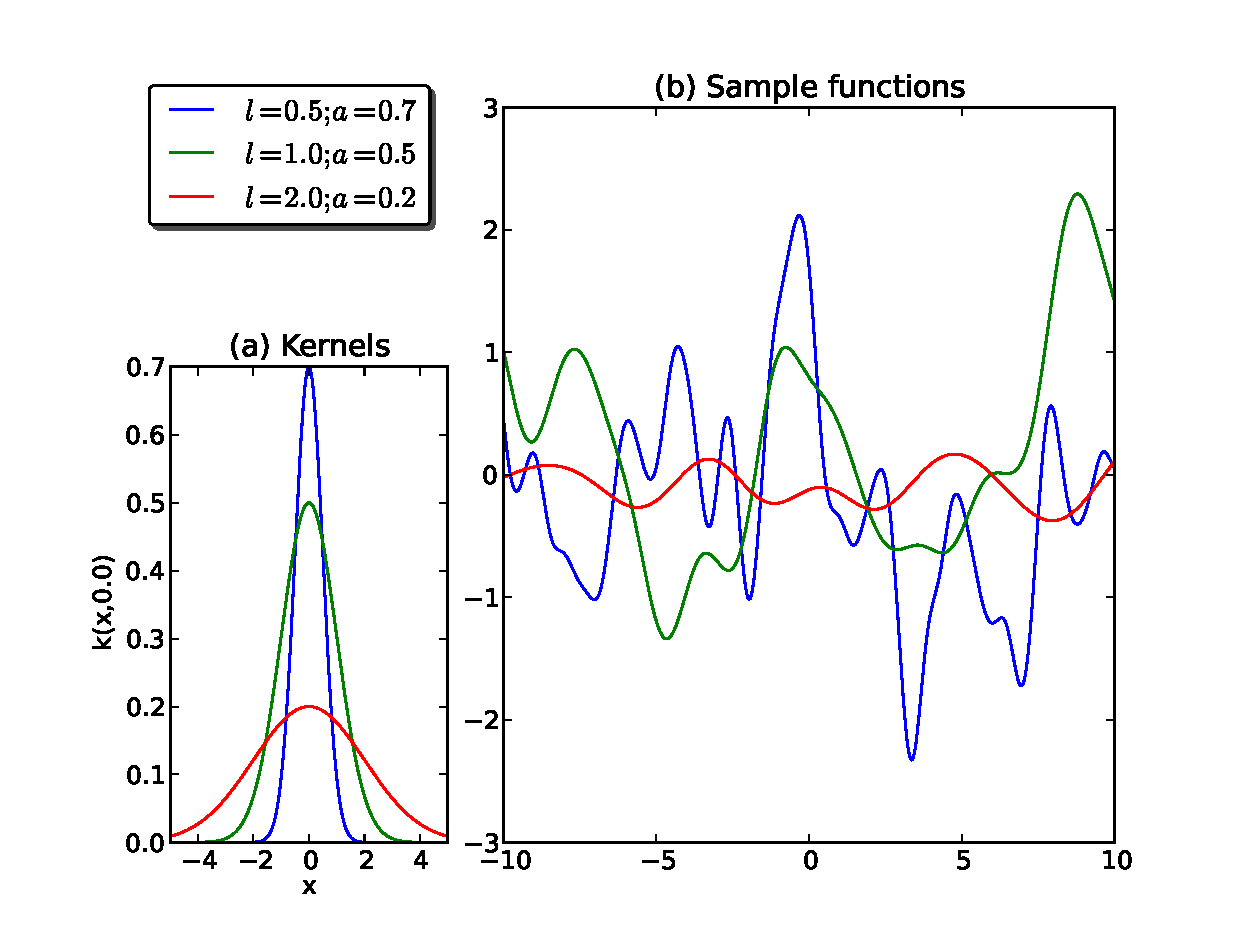
\includegraphics[width=14cm,keepaspectratio]{SE_cov.eps}
		\rule{35em}{0.5pt}
	\caption[Exponentiated Quadratic kernel and sample functions]
		{Exponentiated Quadratic kernel and sample functions}
	\label{fig:Exponentiated_Quadratic_covariance}
\end{figure}
Figure \ref{fig:Exponentiated_Quadratic_covariance}$(a)$ represents the kernel and Figure \ref{fig:Exponentiated_Quadratic_covariance}$(b)$ shows random sample functions drawn from Gaussian process using Exponentiated Quadratic covariance with different lengthscale and amplitude hyperparameter. The random function was generated for a given input range by drawing a sample from the multivariate Gaussian using equation \ref{eq:2.2} with zero mean. The smoothness of the sample function depends on the equation \ref{eq:EQ_cov}. Function variable located closer in the input space are highly correlated, whereas function variable located at distance are loosely correlated or even uncorrelated. Exponentiated Quadratic covariance might be too smooth to perform any realistic regression task. Depending on the basic nature of the function other covariance function could be interesting.

\subsection{Rational Quadratic covariance function}
\begin{figure}
	\centering
		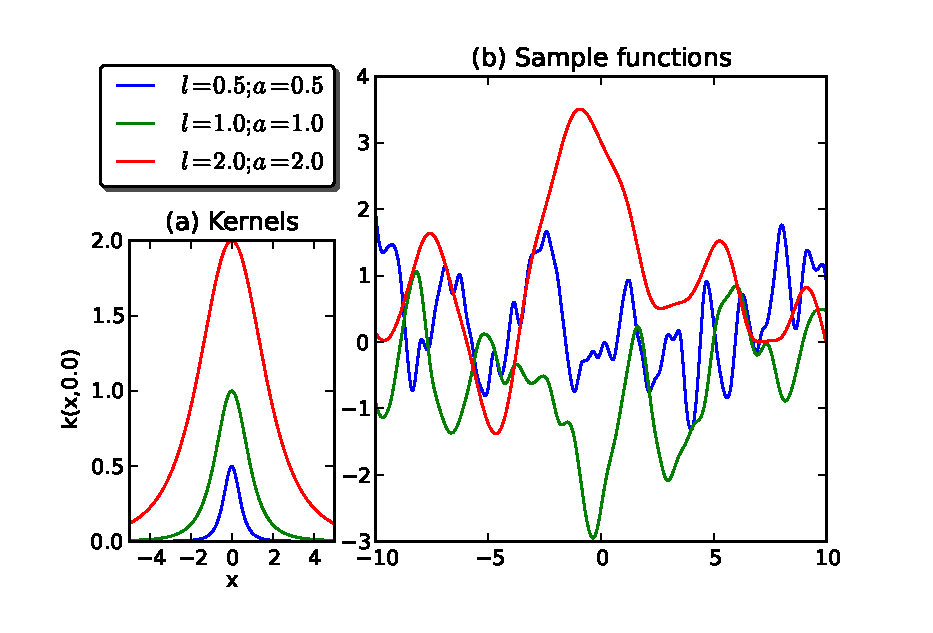
\includegraphics[width=14cm,keepaspectratio]{RQ_edit_cov.eps}
		\rule{35em}{0.5pt}
	\caption[Rational Quadratic kernel and random sample functions]
		{Rational Quadratic kernel and random sample functions}
	\label{fig:Rational_Quadratic_covariance}
\end{figure}
Rational Quadratic covariance function is equivalent to adding together multiple exponentiated quadratic covariance function having different lengthscale. Gaussian process prior kernel function expect smooth function with many lengthscale. Here the parameter $\alpha$ can control the relative weights for lengthscale variations. Exponentiated quadratic covariance function can be viewed as a special case of rational quadratic covariance function. If $\alpha \to \infty$, then both of the functions become identical.

\begin{equation} \label{eq:RQ_cov}
K_{RQ}(r)= a^2 \left(1+ \frac{r^2}{2 \alpha l^2}\right)^{-\alpha}
\end{equation}
where $r=\lVert \textbf{x}-\textbf{x}\textprime \rVert$. Figure \ref{fig:Rational_Quadratic_covariance} (a) shows the kernels and (b) shows three different random sample functions drawn with different setting of hyperparameters $a$ and $l$.

\begin{figure}[t]
	\centering
		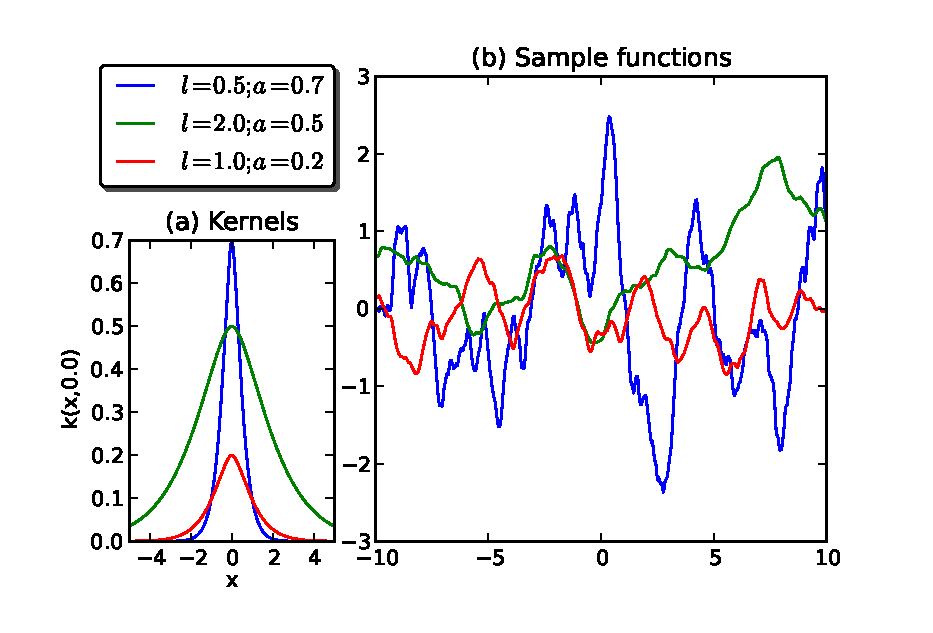
\includegraphics[width=14cm,keepaspectratio]{Mat32_cov.eps}
		\rule{35em}{0.5pt}
	\caption[The Mat{\'e}rn32 kernel and random sample functions]
		{The Mat{\'e}rn32 kernel and random sample functions}
	\label{fig:Matern32_covariance}
\end{figure}


\subsection{The Mat{\'e}rn covariance function}
The Mat{\'e}rn class of covariance function are given by equation \ref{eq:Matern_cov}-
\begin{equation} \label{eq:Matern_cov}
K_{Mat}(r)= a^2\frac{2^{1-\nu}}{\Gamma(\nu)}\left(\frac{\sqrt{2\nu}r}{l}\right)^\nu K_{\nu}
	  \left(\frac{\sqrt{2\nu}r}{l}\right)
\end{equation}
where $a, l, \nu$ are positive hyperparameter, $K_{\nu}$ is a modified Bessel function and $\Gamma \left(.\right)$ is the Gamma function. Hyperparameter $\nu$ controls the roughness of the function and as like Exponentiated quadratic covariance function the parameters $a$ and $l$ controls the amplitude and lengthscale respectively. Though for $\nu \to \infty$ we can obtain the exponentiated quadratic kernel, but for finite value of $\nu$ the sample functions are significantly rough. 

The simpler form of Mat{\'e}rn covariance function is obtained when $\nu$ is half integer: $\nu = p+1/2$, where $p$ is a non-negative integer. The covariance function can be expressed as a product of an exponential and a polynomial of order $p$. \cite{Abramowitz:1965} derived the general expression as follows-
\begin{equation} \label{eq:MaternGeneral}
K_{\nu=p+1/2}(r)= \exp \left( - \frac{\sqrt{2\nu}r}{l}\right)\frac{\Gamma\left(p+1\right)}{\Gamma\left(2p+1\right)}
		\sum_{i=0}^{p}\frac{\left(p+i\right)!}{i!\left(p-i\right)!}
		\left(\frac{\sqrt{8\nu}r}{l}\right)^{p-i}
\end{equation}
The most interesting cases for machine learning are $\nu =3/2$ and $\nu=5/2$, for which we get the following equations respectively-
\begin{equation} \label{eq:Matern32}
K_{\nu=3/2}(r)= \left(1+ \frac{\sqrt{3}r}{l} \right)\exp \left( - \frac{\sqrt{3}r}{l} \right)
\end{equation}
\begin{equation} \label{eq:Matern52}
K_{\nu=5/2}(r)= \left(1+ \frac{\sqrt{5}r}{l} + \frac{5r^2}{3l^2} \right)
		\exp \left( - \frac{\sqrt{5}r}{l} \right)
\end{equation}

\subsection{The Ornstein-Uhlenbeck Process}
\begin{figure}[t]
	\centering
		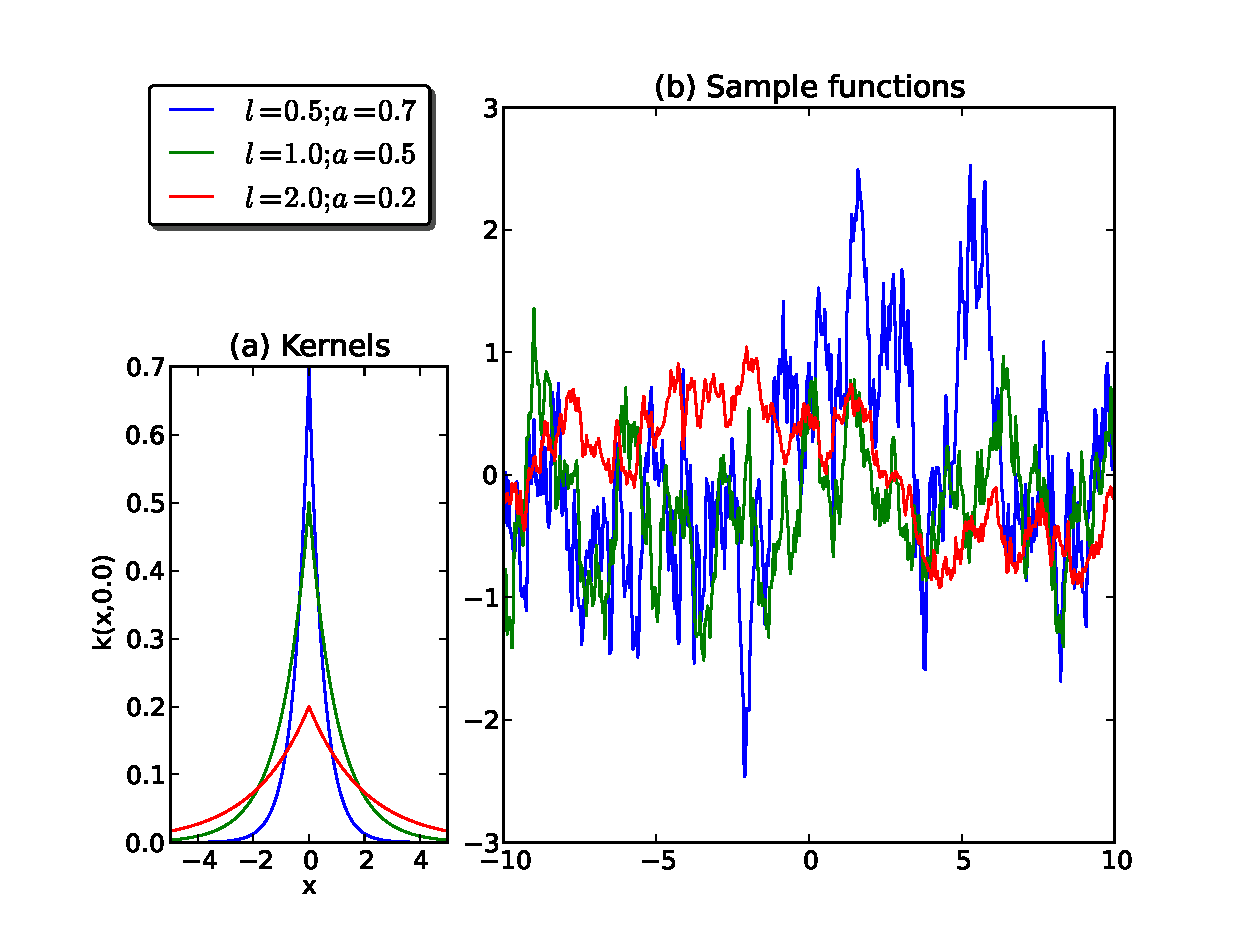
\includegraphics[width=14cm,keepaspectratio]{OU_cov.eps}
		\rule{35em}{0.5pt}
	\caption[The OU kernel and random sample functions]
		{The OU kernel and random sample functions}
	\label{fig:OU_covariance}
\end{figure}
The Ornstein-Uhlenbeck process (\cite{Ornstein_Uhlenbeck:1930}) is a special case of Mat{\'e}rn class covariance functions. The Ornstein-Uhlenbeck (OU) process was developed as a mathematical model of the velocity of a particle moving with Brownian motion.

The OU process can be found setting up $\nu=1/2$ and expressed as Equation \ref{eq:OU}. Figure \ref{fig:OU_covariance}$(a)$ shows the kernel and Figure \ref{fig:OU_covariance}$(b)$ shows the sample functions form the OU process having the exactly same amplitude parameter $a$ and lengthscale parameter $l$.  
\begin{equation} \label{eq:OU}
K_{\nu=1/2}(r)=	\exp \left(-\frac{r}{l} \right)
\end{equation}

\begin{figure}[t]
	\centering
		\includegraphics[width=\textwidth,keepaspectratio]{differentKernels.pdf}
		\rule{35em}{0.5pt}
	\caption[Representation of some basic kernels ]
		{Representation of some basic kernels using the same lengthscale and variance (a). Linear kernel (b). Brownian kernel (c). Exponentiated Quadratic kernel, (d). Cosine kernel (e). Exponential kernel (f). Periodic Exponential kernel}
	\label{fig:DifferentKernels}
\end{figure}

\begin{figure}[t]
	\centering
		\includegraphics[width=\textwidth,keepaspectratio]{ConstructKernels_BR_Cos.pdf}
		\rule{35em}{0.5pt}
	\caption[Construct kernel adding two basic kernels]
		{Construct kernel adding two basic kernels: an example of a univariate data which is globally periodic and locally governed by some random motion. (top-left) sample taken using Brownian kernel, (top-middle) sample taken using Cosine kernel, (top-right) sample taken using newly constructed kernel by adding two kernels, (bottom-left) Brownian kernel, (bottom-middle) Cosine kernel, (bottom-right) newly constructed kernel} %#TODO Explain
	\label{fig:ConstructKernels_BR_Cos}
\end{figure}

\section{Constructing Kernels}
Figure \ref{fig:DifferentKernels} shows the representation of some basic kernels using the same lengthscale and variance (a). Linear kernel (b). Brownian kernel (c). Exponentiated Quadratic kernel, (d). Cosine kernel (e). Exponential kernel (f). Periodic Exponential kernel. These kernels are the 
realization of different covariance function\footnote{We have not describe the Linear, Brownian, Exponential, Periodic Exponential and Cosine kernels here. Detail description is available at \cite{Rasmussen_and_Williams:2006} and their $Python$-based implementation is available at \cite{gpy2014}.}.

There are lots of defined kernels (both stationary and non-stationary) for Gaussian processes to deal with variety of kind of structure. Yet, these kernels might not be enough to express certain kind of structures. Gaussian process facilitate to construct new kernels or customize \lq on demand\rq of the structure with the desired properties. \lq Addition\rq and \lq multiplication\rq' are two simple operations to combining kernels.

Assume in an univariate data is globally periodic and local structure governed by some random motion (Brownian motion). There are multiple choice to deal with the global structure and one of the possible solution could be a Cosine kernel for global structure and a Brownian kernel for local structure in an additive form. Addition of two positive semi-definite kernels together always results another positive semi-definite kernel. Figure \ref{fig:ConstructKernels_BR_Cos} shows the sample functions and representation of the newly constructed kernel.

\begin{figure}[t]
	\centering
		\includegraphics[width=\textwidth,keepaspectratio]{ConstructKernels_Cos_Mat52.pdf}
		\rule{35em}{0.5pt}
	\caption[Construct kernel from two basic kernels ]
		{Construct kernel from two basic kernels} %#TODO Explain
	\label{fig:ConstructKernels}
\end{figure}

\section{Gaussian Process Regression}
Gaussian process regression can be done using the marginal and conditional properties of multivariate Gaussian distribution. Lets consider that we have some observations $\mathbf{f}$ of a function at observation point $\mathbf{x}$. Now we wish to predict the values of that function at observation points $\mathbf{x_\star}$, which we are representing by $\mathbf{f_\star}$. Then the joint probability of $\mathbf{f}$ and $\mathbf{f_\star}$ can be obtained from equation \ref{eq:jointPro_f_f*}-

\begin{equation} \label{eq:jointPro_f_f*}
p \left( \begin{bmatrix} \mathbf{f} \\\mathbf{f_\star} \end{bmatrix} \right) =
\mathcal{N}\left( \begin{bmatrix} \mathbf{f} \\\mathbf{f_\star} \end{bmatrix} \middle|
\mathbf{0}, \begin{bmatrix} \mathbf{K_{x,x}} & \mathbf{K_{x,x_\star}} \\
			    \mathbf{K_{x_\star,x}} & \mathbf{K_{x_\star,x_\star}} \end{bmatrix} \right)
\end{equation}

where the covariance matrix $ \mathbf{K_{x,x}}$ has elements derived from the covariance function $ k \left(x,x\textprime \right)$, such that the $ \left(i,j \right)^{th}$ element of $ \mathbf{K_{x,x}}$ is
given by $k \left( \mathbf{x} \left[ i\right],\mathbf{x} \left[ i\right] \right) $ The conditional property of a multivariate Gaussian is used to perform regression the. The conditional property is can be represented by the equation \ref{eq:condProMvG}: 

\begin{equation} \label{eq:condProMvG}
p \left( \mathbf{f} \middle| \mathbf{f_\star} \right) =
\mathcal{N}\left( \mathbf{f_\star} \middle| \mathbf{K_{x_\star,x}}  \mathbf{K^{-1}_{x,x}} \mathbf{f,} \mathbf{K_{x_\star,x_\star}} - 
\mathbf{K_{x_\star,x}} \mathbf{K^{-1}_{x,x}} \mathbf{K_{x,x_\star}}\right)
\end{equation}

In ideal case the observations $\mathbf{f}$ is noise free but in practice it is always corrupted with some noise. Lets consider $\mathbf{y}$ is the corrupted version of $\mathbf{f}$. If we consider this noise as Gaussian noise then we can write $p \left( \mathbf{y} \middle| \mathbf{f} \right) = \mathcal{N} \left( \mathbf{y} \middle| \mathbf{f}, \sigma^2 \mathbf{I} \right) $, where $ \sigma^2 $ is the variance of the noise and $\mathbf{I}$ is the identity matrix with appropriate size and marginalise the observation $\mathbf{f}$. Then the joint probability of $\mathbf{y}$ and $\mathbf{f_\star}$ can be represented by the equation \ref{eq:jointPro_y_f*}.

\begin{equation} \label{eq:jointPro_y_f*}
p \left( \begin{bmatrix} \mathbf{y} \\\mathbf{f_\star} \end{bmatrix} \right) =
\mathcal{N}\left( \begin{bmatrix} \mathbf{y} \\\mathbf{f_\star} \end{bmatrix} \middle|
\mathbf{0}, \begin{bmatrix} \mathbf{K_{x,x}}+ \sigma^2\mathbf{I} & \mathbf{K_{x,x_\star}} \\
			    \mathbf{K_{x_\star,x}} & \mathbf{K_{x_\star,x_\star}} \end{bmatrix} \right)
\end{equation}

Regression with Gaussian process is Bayesian method. From the knowledge of a $prior$ over a function we proceed to a $posterior$ and this happens in a closed from of equation \ref{eq:condProMvG}. 

\begin{figure}[t]
	\centering
		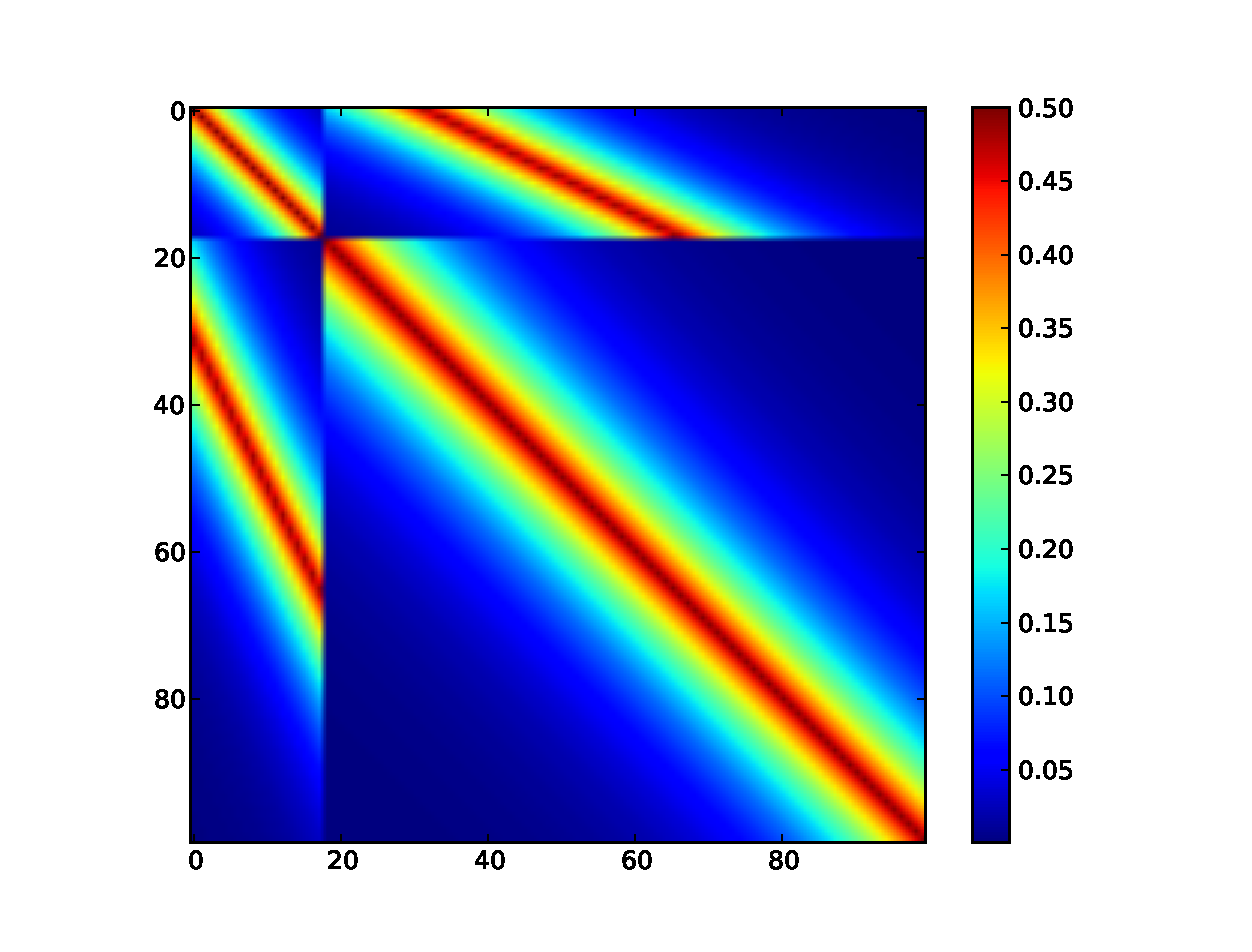
\includegraphics[width=0.8\textwidth,keepaspectratio]{Cov_Structure.eps}
		\rule{35em}{0.5pt}
	\caption[Overall representation of covariances between training and test data]
		{Overall representation of covariances between training and test data}
	\label{fig:Covariances_Structure}
\end{figure}

Figure \ref{fig:Covariances_Structure} shows the overall covariance structure between some training and test data. For this example we choose 18 training points and 82 test points. We observed the shaded structure because some of the training data are closer to some of the test data. Observing this structure we can also figure out the closeness between training and test data. 

\begin{figure}
	\centering
		\includegraphics[width=0.95\textwidth]{regDemo2.pdf}
		\rule{35em}{0.5pt}
	\caption[A visual representation of Gaussian process regression: Modelling a one dimensional function using Gaussian process]
		{A visual representation of Gaussian process regression: Modelling a one dimensional function using Gaussian process. Coloured solid lines represent different samples from the process and dotted line is the mean function. The shaded area is 95\% confidence interval. (a). A Gaussian process not conditioned on any data points. Without any observations, the prior uncertainty about the underlying function is constant everywhere. (b). to (e). The posterior after conditioning on different amount of data.}
	\label{fig:dempGPReg}
\end{figure}

\subsection{Making prediction}
The probability density is represented by functions. Due to consistency this density is known as a process. Also by this property, any future values of $\mathbf{f_\star}$ which are unobserved can be predicted without affecting $\mathbf{f}$. To make prediction of the test data we use the conditional distribution. In ideal case the conditional distribution is $ p\left( \mathbf{f_\star} \middle| \mathbf{f} \right) $ and if we consider the noise then the conditional distribution will be $ p\left( \mathbf{f_\star} \middle| \mathbf{y} \right) $. Both of the distribution are also Gaussian,
\begin{equation} \label{eq:prediction}
  \mathbf{f_\star}  \sim \left( \boldsymbol{\mu}_f, \mathbf{C}_f \right)
\end{equation}

The mean of the conditional distribution of Equation \ref{eq:prediction} is:
\begin{equation} \label{eq:prediction_mean}
  \boldsymbol{\mu}_f = \mathbf{K_{x,x_\star}^T} \left[ \mathbf{K_{x,x}}+ \sigma^2\mathbf{I} \right]^{-1} \mathbf{y}
\end{equation}

and the covariance of the conditional distribution of Equation \ref{eq:prediction} given by:
\begin{equation} \label{eq:prediction_cov}
  \mathbf{C}_f = \mathbf{K_{x_\star,x_\star}} -
		\mathbf{K_{x,x_\star}^T} \left[ \mathbf{K_{x,x}}+ \sigma^2\mathbf{I} \right]^{-1} \mathbf{K_{x,x_\star}}
\end{equation}

These results can be calculated using block matrix inverse rules. The derivation can found in appendix section ({\color{red} Appendix \ref{AppendixA}}). Figure \ref{fig:dempGPReg} shows a visual representation of Gaussian process regression for a one dimensional function. Coloured solid lines represent different samples from the process and dotted line is the mean function. The shaded area is 95\% confidence interval. (a) of Figure \ref{fig:dempGPReg} represent a Gaussian process not conditioned on any data points. Without any observations, the prior uncertainty about the underlying function is constant everywhere. (b). to (e). of Figure \ref{fig:dempGPReg} shows some posterior samples after conditioning on different amount of data. 

%TODO


\subsection{Hyperparameter Learning}
To construct the covariance function still we need to consider the hyperparameters and optimize those. These adjustable parameters alter the distribution of the function output values obtained from a Gaussian process. The most efficient and commonly used optimization technique for hyperparameters can be done using maximum likelihood. If we consider all the hyperparameters $\alpha$, $\sigma^2$ and $l$ in to a vector $\boldsymbol{\theta}$, then we can use gradient methods to optimize $p \left(\mathbf{y}\middle|\boldsymbol{\theta}\right)$ with respect to $\boldsymbol{\theta}$. The Log likelihood is given by:

\begin{equation} \label{eq:Likelihood}
 p \left(\mathbf{y}\middle|\boldsymbol{\theta}\right) =
    - \frac{D}{2}log2\pi - \frac{1}{2}\times log \left| \mathbf{K_{x,x}} + \sigma^2\mathbf{I}\right|
    - \frac{1}{2}\mathbf{y}^T \left[\mathbf{K_{x,x}} + \sigma^2\mathbf{I} \right]^{-1}\mathbf{y}
\end{equation}

We can have the Log maximum likelihood by:
\begin{equation} \label{eq:LML}
 \boldsymbol{\theta}_{max} = argmax \left( p\left(\mathbf{y}\middle|\boldsymbol{\theta}\right) \right)
\end{equation}

% TODO Andreas 15

\section{Toward the GP model of TFA}
 We are interested to develop a non-parametric model of transcription factor activity using Gaussian process. Here, we want to prove that there is an analogical pathway\footnote{We would like to acknowledge Simo S\"arkk\"a, Academy Research Fellow, Aalto University, Finland for his valuable suggestions and guidelines.} to construct a kernel function for Gaussian process model from Markovian assumption based probabilistic approach of \cite{Sanguinetti:2006}. From Chapter \ref{ch:Probabilistic_TFA} Section \ref{sec:Probabilistic_TFA} we have the probabilistic gene specific TFAs as-
\begin{equation} \label{eq:tfa_SanG_updateCh4}
  \bold{b}_{n(t+1)} \sim \mathcal{N} (\gamma \bold{b}_{nt} + (1-\gamma)\boldsymbol{\mu},(1-\gamma^2)\bold{\Sigma})
\end{equation}
For a discrete time variable $k$ the above equation can be rewrite as-
\begin{equation}
\textbf{b}_{n(k+1)} \sim \mathcal{N}\left(\gamma \textbf{b}_{nk} + (1 - \gamma) \boldsymbol{\mu}, (1 - \gamma^2) \boldsymbol{\Sigma}\right),
\end{equation}
and
\begin{equation}
\textbf{b}_{n_1} \sim \mathcal{N}\left(\boldsymbol{\mu}, \boldsymbol{\Sigma}\right)
\end{equation}
Let's now form a continuous model which has these same finite-dimensional distributions. First construct a one-dimensional process with the property-
\begin{equation}
u_{k+1} \sim \mathcal{N}\left(\gamma u_k + \left(1 - \gamma\right) \mu, (1 - \gamma^2)s \right),
\end{equation}
where $\mu$ and $s$ are scalar.

We can now assume that $u_k$'s are actually values $u_{t_k}$ from a continuous process $u(t)$ and let's assume that- 
\begin{equation}
t_k = kDt.
\end{equation}

A good candidate for this kind of model is the mean-reverting $Ornstein-Uhlenbeck$ model 
(\cite{Ornstein_Uhlenbeck:1930})-
\begin{equation}
du = -\lambda \left(u - \mu\right) dt + q^{1/2} dB,
\end{equation}
where $B$ is a standard Brownian motion (i.e., Wiener process). This equation can now be solved on the time instants $t_k$ and the result is a recursion
\begin{equation}
u(t_k) = a u(t_{k-1}) + b \mu + w_{k-1},
\end{equation}
where $w_{k-1} \sim \mathcal{N}(0,c)$ with-\\
$a = \exp(-\lambda Dt)$\\~\\
$b = \int_0^Dt \exp(-\lambda (Dt-s)) ds\\
 = 1 - \exp(-\lambda Dt)$\\~\\
$c = \int_0^Dt \exp(-\lambda (Dt-s)) q \exp(-\lambda (Dt-s)) ds \\
= q \int_0^Dt \exp(-2 \lambda (Dt-s)) ds\\
= [q / (2 \lambda)] [1 - \exp(-2 \lambda Dt)]$

That is,
\begin{equation}
u_{k+1} \sim \mathcal{N}\left(a u_k + b \mu, c\right).
\end{equation}

We can now match the coefficients:
\begin{equation} \label{eq:a}
a = \exp(-\lambda Dt) = \gamma
\end{equation}
\begin{equation} \label{eq:b}
b = 1 - \exp(-\lambda Dt) = 1 - \gamma
\end{equation}
\begin{equation} \label{eq:c}
c = (1 - \gamma^2) s = [q / (2 \lambda)] [1 - \exp(-2 \lambda Dt)]
\end{equation}

Equation \ref{eq:a} quite luckily has a nice solution 
$\gamma = \exp(-\lambda Dt)$ and from Equation \ref{eq:c} we will have another solution
$s = q / (2 \lambda)$,
which can be inverted to give
$\lambda = -[1 / Dt] \log \gamma$ and
$q = -[2 s / Dt] \log \gamma$. 

If we arbitrarily fix $Dt = 1$, we get
$\lambda = -\log \gamma$\\
$q = -2 s \log \gamma$.

We can now recall that the (stationary) covariance function of the Ornstein-Uhlenbeck process we get-

$k_u(t,t')
  = [q / (2 \lambda)] \exp(-\lambda {\left|t-t'\right|})\\
  = s \exp((\log \gamma) {\left|t-t'\right|})\\
  = s \exp({\left|t-t'\right|}(\log \gamma))\\
  = s \exp(\log \gamma^{\left|t-t'\right|})\\
  = s \gamma^{\left|t-t'\right|}$.

When we start from variance $s = q / \left[2 \lambda\right]$, then the process will indeed be stationary from the start. Returning to the original vector valued $\textbf{b}$, because the system is separable, we can conclude that the implied covariance function is just obtained by formally replacing $s$ with $\boldsymbol{\Sigma}$ everywhere- 
\begin{equation}
\textbf{K}_b(t,t') = \boldsymbol{\Sigma} \boldsymbol{\gamma}^{\left|t-t'\right|}
\end{equation}

Thus is equivalent to considering the vector process of mean-reverting $Ornstein-Uhlenbeck$ model
\begin{equation}
\textbf{db} = -\lambda (\textbf{b} - \boldsymbol{\mu}) \textbf{dt} + Q^{1/2} \textbf{dB}.
\end{equation}

\section{Gaussian Process: Pros and Cons}
The most appealing feature of Gaussian process is expressibility. It is possible to express a very wide range of modelling assumption through a proper choice of covariance function. Given a covariance function and some observations, the posterior distribution can be predicted exactly. Modelling with Gaussian process is non-parametric and this is a rare property. The marginal likelihood of the data given a model is calculated by integrating over all hypothesis. Thus Gaussian process compare different models and improve the model selection. Integration over a wide range of hypothesis lessen over-fitting than in comparable model class. The predictive distribution of Gaussian Process is a multivariate Gaussian distribution and can be easily composed with other models.

There are several issues which may make Gaussian processes sometimes difficult to use. The generic inference and learning algorithm where we need to inverse the matrix has $\mathcal{O}\left(N^3\right)$ runtime complexity. Given the computational resource available at present, the exact inference is prohibitively slow for more than a few thousands data-points. An exact inference for typical \lq Big Data\rq  could be nightmare. However, this problem can be addressed by variational inference, even for the models containing millions of data points (\cite{Hensman:2013a}). Non-Gaussian predictive likelihoods and sparse approximations could be challenging while working with Gaussian process. However, Gaussian process framework GPy (\cite{gpy2014}) can automatically deal with both of the issues. 

\section{Discussion}
%TODO